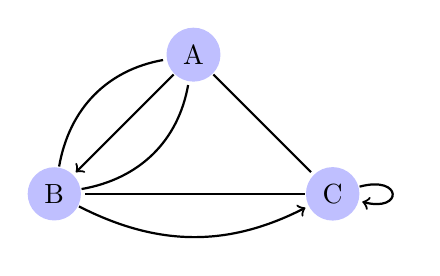
\begin{tikzpicture}[shorten >=1pt,auto,node distance=2.5cm,  
                thick,main node/.style={circle,fill=blue!25}]
                                                             
  \node[main node] (a) {A};                                  
  \node[main node] (b) [below left of=a] {B};                
  \node[main node] (c) [below right of=a] {C};               
                                                             
    \path [->] (a) edge node {} (b);                         
    \path      (a) edge node {} (c);                         
    \path      (b) edge [bend left=35] node {} (a);          
      \path      (b) edge [bend right=35] node {} (a);       
    \path [->] (b) edge [bend right=27] node {} (c);         
    \path      (c) edge [loop right] node {} (c);            
    \path      (c) edge node [above] {} (b);                 
\end{tikzpicture}
